\documentclass[11pt,a4paper]{article}

\usepackage[margin=1in]{geometry}
\usepackage[T1]{fontenc}
\usepackage[utf8]{inputenc}
\usepackage{lmodern}
\usepackage{amsmath,amssymb}
\usepackage{graphicx}
\usepackage{booktabs}
\usepackage{multirow}
\usepackage[authoryear,round]{natbib}
\usepackage{url}
\usepackage[hidelinks]{hyperref}
\usepackage[capitalise,noabbrev]{cleveref}
\usepackage{microtype}
\setlength{\emergencystretch}{2em}

% Short label names (full official names are given in Section 1.1)
\newcommand{\EQ}{\textsc{Eq}}
\newcommand{\FWD}{\textsc{Fwd}}
\newcommand{\BWD}{\textsc{Bwd}}
\newcommand{\NEG}{\textsc{Neg}}
\DeclareMathOperator{\rev}{rev}

\title{Directional Consistency in Fine-Grained NLI:\\
Problem Formulation, Exploratory Analysis and Baselines for DiCo-NLI (Track~1)\\[4pt]
\large CS-878 Deep Learning, Assignment 1}
% TODO: add all team members' names as required by the course.
\author{Muneeb Baig\\ MS Data Science, SEECS, NUST}
\date{\today}

\begin{document}
\maketitle

% =====================================================================
\section{Introduction and Task Definition}
\label{sec:intro}

Natural Language Inference (NLI) is a standard test of whether models can identify semantic relations between texts. A model can score well on NLI benchmarks by exploiting superficial cues in the data \citep{gururangan2018annotation}. Standard evaluation also scores each ordered pair on its own, so it cannot show whether a model's judgements stay coherent when the same pair is presented in the opposite order.

DiCo-NLI (SemEval-2027 Task~2) addresses the second problem \citep{diconli2026}. Systems classify the relation between two short phrases, and every reversible pair is evaluated in both orders, so classification quality and directional consistency are measured together \citep{apaolaza2026assessing}.

We work on Track~1 (English). We start with an analysis of the data, looking for cues a model could use and for cues it could exploit without understanding the relation. We then train classical baselines, some of them deliberately restricted to phrase length or lexical overlap, and finally fine-tune BERT and RoBERTa. Every system is scored with the official metrics: Weighted F1, SoftCons and HardCons.

\paragraph{Research question.} How far can shallow structural cues and standard fine-tuned encoders progress on DiCo-NLI, and to what extent does directional consistency reflect correct relational classification?

\paragraph{Hypotheses.}
\textbf{H1:} Surface cues such as phrase length yield non-trivial classification performance and high SoftCons.
\textbf{H2:} Fine-tuned cross-encoders outperform the classical baselines on Weighted F1 and HardCons.
\textbf{H3:} The remaining errors of the fine-tuned encoders concentrate at the boundary with \NEG{} rather than on inference direction.

\subsection{Task definition: black-box view}
\label{sec:task}

Each instance is an ordered pair of short phrases $x=(t_1,t_2)$, and the system predicts one of four labels: \texttt{EQUIVALENCE}, \texttt{FORWARD\_ENTAILMENT}, \texttt{BACKWARD\_ENTAILMENT} and \texttt{NEGATIVE\_OTHER} \citep{diconli2026}, abbreviated in the rest of this report as $\mathcal{Y}=\{\EQ,\FWD,\BWD,\NEG\}$. The labels can be read as answers to two questions: does $t_1$ entail $t_2$, and does $t_2$ entail $t_1$?
\EQ{} holds when $t_1 \Rightarrow t_2$ and $t_2 \Rightarrow t_1$;
\FWD{} when $t_1 \Rightarrow t_2$ but $t_2 \not\Rightarrow t_1$;
\BWD{} when $t_2 \Rightarrow t_1$ but $t_1 \not\Rightarrow t_2$.
\NEG{} groups all remaining relations of the source benchmark (opposition, similarity, relatedness and unrelatedness) into a single label \citep{diconli2026}.

The direction of the input is therefore part of the prediction. For example, the training pair ``Japanese PM Shinzo Abe'' $\rightarrow$ ``Abe'' is labelled \FWD; reversing the two phrases yields \BWD. An equivalent pair such as ``a monochrome photograph'' and ``a black and white photo'' remains \EQ{} after reversal, whereas ``in southern Iraq'' and ``in northern Iraq'' belong to \NEG.

Formally, for the reversible labels we define the reversal operator
\begin{equation}
\rev(\FWD)=\BWD,\qquad \rev(\BWD)=\FWD,\qquad \rev(\EQ)=\EQ .
\end{equation}
A directionally coherent classifier $f$ should satisfy, for every reversible pair,
\begin{equation}
\label{eq:coherence}
f(t_2,t_1)=\rev\big(f(t_1,t_2)\big).
\end{equation}
\NEG{} instances occur in one orientation only and are excluded from the pair-level consistency metrics; however, predicting \NEG{} for either member of a reversible pair breaks \cref{eq:coherence} and is counted as inconsistent.

\subsection{Task definition: white-box view}

The output is a single four-way label, but the task is harder than that suggests. \FWD{} and \BWD{} differ only in direction, so any signal that stays the same when $t_1$ and $t_2$ are swapped, such as lexical overlap or cosine similarity, cannot tell them apart. High similarity is not equivalence either: ``A sheep'' and ``A large sheep'' share almost everything, yet the added modifier makes the relation one-directional. \NEG{} adds a different difficulty, since it merges several relations into one label and is internally heterogeneous. And because the phrases are only a few words long, a single modifier often decides the label, with little surrounding context to help.

The short length of the phrases also creates a risk. A more specific phrase usually carries extra modifiers and is therefore longer than the phrase it entails, so a classifier could learn to follow length or containment without modelling the relation at all. We check for this shortcut in the exploratory analysis (\cref{sec:eda}) and test it directly with restricted baselines (\cref{sec:baselines}).

% =====================================================================
\section{Related Work}
\label{sec:related}

\paragraph{Shortcuts in NLI data.}
\citet{gururangan2018annotation} showed that NLI datasets contain annotation artifacts: classifiers that see only the hypothesis reach about 67\% accuracy on SNLI and 53\% on MultiNLI, far above the 33\% chance level. We borrow the idea: our restricted baselines see only phrase length or lexical overlap, which shows how much of the task these cues solve on their own.

\paragraph{Phrase-level inference data.}
DiCo-NLI is derived from PhrasIS \citep{lopezgazpio2024phrasis}, a benchmark of over 10{,}000 naturally occurring phrase pairs from image captions and news headlines, annotated by experts for inference relations and semantic similarity. PhrasIS builds on the interpretable semantic textual similarity line of work, in which sentence pairs are decomposed into aligned chunks \citep{lopezgazpio2017interpretable}, and evaluates semantic representations at a finer granularity than sentence-level NLI. At this granularity, small lexical or structural differences between short phrases can change the direction of inference. DiCo-NLI retains the reversible relations \EQ, \FWD{} and \BWD, and maps all other PhrasIS relations to \NEG{} \citep{diconli2026}. \NEG{} is therefore a comparatively heterogeneous category, which may make it harder to separate from the positive relations.

\paragraph{Directionality and the Reversal Curse.}
\citet{berglund2024reversal} showed that autoregressive language models trained on a fact stated in one direction (``A is B'') often fail to answer the reversed query (``B is A''), so directional generalisation cannot be taken for granted. \citet{wu2024reversal} report that this behaviour depends on architecture: in their setting the bidirectional encoder BERT was immune to the reversal curse, although both BERT- and GPT-style models struggled with more complex deductive reasoning over three sets. The Reversal Curse is about retrieving a learned fact backwards. DiCo-NLI asks something narrower \citep{diconli2026}: when the two phrases of a pair swap places, does the predicted relation change in the way the reversal requires?

\paragraph{Coherence-based evaluation.}
The most direct predecessor of DiCo-NLI is the pilot study of \citet{apaolaza2026assessing}, which evaluates logical coherence under reversed inference direction on PhrasIS phrase pairs. They introduce soft and hard causal coherence (SoftCoh and HardCoh): soft coherence measures whether predictions for the two orientations are mutually compatible, while hard coherence additionally requires both predictions to be correct. DiCo-NLI adopts these measures as SoftCons and HardCons. Across 17 encoder, decoder and encoder--decoder Transformers, encoders (in particular DeBERTa-v3) were strongest, and coherence fell by roughly 0.10--0.20 for encoders from seen to unseen phrase pairs. Errors were linked to surface similarity and lexical overlap and to prepositions. The authors also note that coherence does not imply correctness, because a model can be consistently wrong in both directions, and that gold labels can be ambiguous.

\paragraph{Positioning.}
The pilot study used extensively tuned pretrained models on PhrasIS. Our question is more basic: how far do simple structural, lexical and standard fine-tuned baselines get on the official DiCo-NLI split, and how much of their consistency comes from shallow cues? Reporting classification and consistency side by side is what makes the second part answerable.

% =====================================================================
\section{Dataset}
\label{sec:dataset}

\subsection{Data and splits}
We use the official English data of Track~1, derived from PhrasIS \citep{diconli2026}. The training set contains 3{,}042 rows corresponding to 1{,}760 underlying pairs (\texttt{pair\_id}s), and the development set contains 660 rows corresponding to 383 pairs. The reference files additionally provide \texttt{reverse\_pair\_id}, which links the two orientations of each reversible pair and is used to compute the consistency metrics. We use the official splits unchanged. The trial data is not used because it overlaps with the training and development data.

\subsection{Integrity checks}
No missing or empty texts were found, and no \texttt{pair\_id} occurs in both training and development. Otherwise one orientation of a pair could sit in training and its reversal in development, which would leak the answer. Across training and development combined, 116 rows are duplicated, and only one pair carries conflicting labels. Seven development rows have an exact ordered $(t_1,t_2)$ match in the training data despite the absence of \texttt{pair\_id} overlap; we keep the official split but treat this small overlap as a limitation.

\subsection{Label distribution}
The label distribution is nearly identical in both splits: \FWD{} and \BWD{} each account for about 29\% of rows, \EQ{} for about 26\% and \NEG{} for about 16\%. \FWD{} and \BWD{} are balanced by construction, because each reversible entailment pair appears in both orientations, whereas \NEG{} rows have no reversed counterpart. The imbalance is moderate, but because \NEG{} is the smallest class we report Macro F1 alongside the official Weighted F1, so that performance on the less frequent class remains visible.

% =====================================================================
\section{Exploratory Data Analysis}
\label{sec:eda}

We analyse a small set of task-relevant feature groups: phrase length, lexical overlap and containment, part-of-speech (POS) patterns, semantic similarity, and vocabulary coverage. For each group we separate the observation from its interpretation and its modelling implication. All selected plots are provided in a separate EDA PDF; the two most informative are reproduced in \cref{fig:length,fig:containment}.

\subsection{Phrase length and direction}
\textbf{Observation.} For \FWD{}, $t_1$ contains on average 3.58 tokens versus 2.44 for $t_2$, and \BWD{} mirrors this pattern. About 77\% of \FWD{} rows place the longer phrase first, with the reverse for \BWD{}; \EQ{} and \NEG{} have a mean signed length difference of zero (\cref{fig:length}). About 19\% of rows contain at least one single-word phrase.
\textbf{Interpretation.} A more specific phrase often carries additional lexical material and is longer than the more general phrase it entails. Length carries information about direction, although it is only a surface cue.
\textbf{Modelling implication.} Signed length difference should be tested explicitly as a potential shortcut: \cref{sec:features} introduces directional length features and \cref{sec:baselines} evaluates a length-only baseline.

\begin{figure}[t]
\centering
\includegraphics[page=2,width=0.72\linewidth]{figures/eda_plots.pdf}
\caption{Distribution of the signed token-length difference $L(t_1)-L(t_2)$ per label (train and development). \FWD{} and \BWD{} are mirror images; \EQ{} and \NEG{} are centred on zero.}
\label{fig:length}
\end{figure}

\subsection{Lexical overlap and containment}
\textbf{Observation.} In about 45\% of entailment rows the word set of one phrase is fully contained in the other (\cref{fig:containment}). Mean Jaccard similarity is about 0.41 for \FWD{} and \BWD{}, 0.27 for \NEG{} and only 0.24 for \EQ.
\textbf{Interpretation.} Entailment often arises when one phrase adds information to the other, so directional containment is informative. Equivalent phrases, by contrast, frequently express the same meaning with different words. Jaccard similarity is also symmetric, $J(t_1,t_2)=J(t_2,t_1)$, so it cannot by itself distinguish \FWD{} from \BWD.
\textbf{Modelling implication.} We separate directional containment features from symmetric overlap features and evaluate a symmetric-overlap-only probe.

\begin{figure}[t]
\centering
\includegraphics[page=5,width=0.72\linewidth]{figures/eda_plots.pdf}
\caption{Word-set containment pattern per label (row-normalised). One-sided containment is characteristic of \FWD{} and \BWD{}; \EQ{} and \NEG{} pairs rarely contain one another.}
\label{fig:containment}
\end{figure}

\subsection{Part-of-speech patterns}
We examine the POS of words that occur in only one side of a pair.
\textbf{Observation.} Compared with the other labels, words found only in $t_1$ of \FWD{} pairs are especially often adjectives (0.39 per pair vs.\ 0.16 for \EQ) and proper nouns (0.24 vs.\ 0.11), with the mirror pattern in $t_2$ for \BWD. \EQ{} and \NEG{} pairs also contain many non-shared nouns (about 0.57 per side), but on both sides, which is characteristic of lexical substitution rather than one-sided addition. Across all tokens, \NEG{} phrases also contain the highest proportion of prepositions (17.4\%, compared with 12.9\% for the entailment classes), consistent with contrastive pairs such as ``to hospital'' / ``from hospital'' (a \NEG{} training pair).
\textbf{Interpretation.} Adjectives and named-entity detail make a phrase more specific while preserving entailment of the more general phrase, so their directional distribution carries information about direction.
\textbf{Modelling implication.} We add directional POS counts of non-shared words to the engineered features.

\subsection{Semantic similarity}
Each phrase is encoded independently with a frozen MiniLM sentence encoder (\texttt{all-MiniLM-L6-v2}) and the cosine similarity of the two embeddings is computed.
\textbf{Observation.} Mean cosine similarity is about 0.74 for \FWD{} and \BWD, 0.72 for \EQ{} and 0.62 for \NEG.
\textbf{Interpretation.} Similarity separates related from unrelated pairs, but it does not identify the direction or the exact type of relation. Cosine similarity is symmetric, $\cos(\mathbf{e}_1,\mathbf{e}_2)=\cos(\mathbf{e}_2,\mathbf{e}_1)$, and therefore direction-blind; the near-identical values for \EQ{} and the entailment labels also show that similarity is not the same as inference.
\textbf{Modelling implication.} A model needs to read the ordered pair jointly, so our pretrained baselines are pair encoders.

\subsection{Vocabulary sparsity}
\textbf{Observation.} About 47\% of training vocabulary types occur only once, and 15.4\% of development tokens are out of vocabulary with respect to the training data.
\textbf{Interpretation.} Representations built only from training-set word identities have little or no evidence for rare and unseen words.
\textbf{Modelling implication.} We compare a TF--IDF lexical baseline with pretrained encoders, whose subword tokenisation and pretraining provide information about such words.

\paragraph{Summary.} Length, containment, adjectives and proper nouns all point in the direction of entailment, and some of them are cheap enough to be shortcuts. Jaccard overlap and cosine similarity look informative at first, but both are symmetric, so neither can separate \FWD{} from \BWD{} by itself. The features in \cref{sec:features} and the diagnostic baselines in \cref{sec:baselines} follow directly from these observations.

% =====================================================================
\section{Feature Engineering}
\label{sec:features}

Guided by the EDA, we construct 26 numerical features for each ordered pair. Besides providing a classical baseline representation, they are designed to separate directional signals from symmetric ones.

\paragraph{Length (4).} Token counts of $t_1$ and $t_2$, the signed token-length difference $L(t_1)-L(t_2)$, and the signed character-length difference. The signed differences change sign when the pair is reversed.

\paragraph{Symmetric overlap (2).} Jaccard similarity of the two word sets and an indicator for identical texts. Both are unchanged under reversal.

\paragraph{Directional coverage and containment (6).} The proportion of $t_1$'s words found in $t_2$ and vice versa, binary full-containment indicators in both directions, and the numbers of words occurring only in $t_1$ and only in $t_2$. Unlike Jaccard similarity, these features indicate which phrase contains the additional material.

\paragraph{Task-specific cues (2).} Negation mismatch is 1 when exactly one phrase contains a negation term (\emph{not, no, never, n't, without, none, nobody, nothing}). Number mismatch is 1 when the sets of digit tokens differ. Because it considers digit tokens only, it does not normalise written and numeric forms such as ``Two'' and ``2''; this is a limitation of the deliberately simple feature.

\paragraph{POS of non-shared words (12).} Using spaCy (\texttt{en\_core\_web\_sm}), we count NOUN, PROPN, ADJ, VERB, ADP and NUM tokens among the words that occur in only one phrase, separately for $t_1$ and $t_2$.

\paragraph{Directionality and preprocessing.} Most features are directional: under reversal, signed quantities change sign and phrase-specific features exchange roles. Only Jaccard similarity and the identical-text indicator are symmetric; \cref{sec:baselines} exploits this distinction through separate diagnostic probes. The 26 features are standardised with $z$-score parameters fitted on the training data, which also makes the logistic-regression coefficients comparable. The MiniLM similarity of \cref{sec:eda} is used only for exploration and is not a classifier input.

% =====================================================================
\section{Baseline Models}
\label{sec:baselines}

The models go from deliberately weak diagnostic probes up to fully fine-tuned pretrained encoders. The weak end tells us how much of the score simple dataset cues already explain, so that the gains of the stronger models can be read against it.

\subsection{Baseline A: classical models}
All logistic-regression (LR) classifiers use scikit-learn with at most 5{,}000 iterations, the default regularisation $C=1$, and a fixed random state.
\begin{itemize}
  \item \textbf{Majority.} Predicts the most frequent training label. \FWD{} and \BWD{} are tied at 881 training rows; the implementation resolves the tie to \FWD.
  \item \textbf{LR, length only.} Uses only the four length features, to quantify how much classification and consistency the length cue alone provides.
  \item \textbf{LR, symmetric overlap only.} Uses only Jaccard similarity and the identical-text indicator. Since both satisfy $g(t_1,t_2)=g(t_2,t_1)$, this model has no representation of direction and serves as a direction-blind probe.
  \item \textbf{LR, engineered features.} Uses all 26 standardised features.
  \item \textbf{TF--IDF + LR.} Unigram and bigram TF--IDF with sublinear term frequency, with the vocabulary fitted on training phrases only. The two phrases are vectorised separately and concatenated, $\mathbf{x}=[\mathrm{tfidf}(t_1)\,\Vert\,\mathrm{tfidf}(t_2)]$, so that phrase order is retained.
  \item \textbf{TF--IDF + features + LR.} Concatenates the TF--IDF representation with the 26 standardised features.
\end{itemize}

\subsection{Baseline B: fine-tuned pretrained encoders}
We fine-tune \texttt{bert-base-uncased} and \texttt{roberta-base}, each with a new four-way classification head; all encoder weights are updated (no frozen features). Both models are cross-encoders that read the two phrases jointly and in order: BERT receives $[\mathrm{CLS}]\,t_1\,[\mathrm{SEP}]\,t_2\,[\mathrm{SEP}]$ with segment IDs (\texttt{token\_type\_ids}) marking the two phrases, while RoBERTa uses $\langle s\rangle\,t_1\,\langle/s\rangle\langle/s\rangle\,t_2\,\langle/s\rangle$ without segment IDs. Unlike symmetric similarity measures, these encoders can learn order-dependent representations.

The maximum sequence length is 64 tokens and the batch size 16. We use AdamW with learning rate $3\times10^{-5}$, weight decay 0.01, gradient clipping at 1.0 and a linear schedule with 10\% warm-up, and train for six epochs. The final epoch is used, a rule fixed in advance; there is no early stopping and no selection of the best development epoch. Each model is trained with three seeds (13, 42, 87) on an Apple M4 GPU via PyTorch's MPS backend, and we report the mean and standard deviation.

\paragraph{Implementation note.} In a preliminary run the BERT batching pipeline omitted \texttt{token\_type\_ids}, and the training schedule (four epochs, learning rate $2\times10^{-5}$) left the training loss far from converged. Both issues were corrected once, after which the configuration above was frozen. The decision was based on the implementation error and the training loss, not on development-set scores.

% =====================================================================
\section{Evaluation Setup}
\label{sec:evaluation}

All systems are evaluated on the official development set (660 rows) with the organisers' scorer. Of these rows, 554 form $M=277$ reversible pairs (190 \FWD/\BWD{} pairs and 87 \EQ{} pairs), and 106 are \NEG{} rows without a reversed counterpart. We evaluate row-level classification separately from pair-level directional consistency.

\subsection{Classification metrics}
For each class $c$, precision, recall and F1 are
\begin{equation}
P_c=\frac{TP_c}{TP_c+FP_c},\qquad R_c=\frac{TP_c}{TP_c+FN_c},\qquad F1_c=\frac{2P_cR_c}{P_c+R_c}.
\end{equation}
The official classification metric is Weighted F1,
\begin{equation}
\mathrm{W\text{-}F1}=\sum_{c\in\mathcal{Y}}\frac{n_c}{N}\,F1_c ,
\end{equation}
where $n_c$ is the number of development rows with gold label $c$ and $N=660$. Each class contributes in proportion to its support: \NEG{} receives a weight of about 0.16 and the other labels about 0.26--0.29 each. We also report Macro F1, $\frac{1}{|\mathcal{Y}|}\sum_c F1_c$, which gives every class a weight of 0.25. Because \NEG{} is both the smallest class and empirically a difficult one, Weighted F1 gives it less influence than Macro F1 does, and the gap between the two reveals how much a model struggles on this class. Accuracy is reported as a complementary statistic.

\subsection{SoftCons}
Let $\hat y_{i,1}$ and $\hat y_{i,2}$ be the predictions for the two orientations of reversible pair $i$. Then
\begin{equation}
\mathrm{SoftCons}=\frac{1}{M}\sum_{i=1}^{M}\mathbb{1}\!\left[\hat y_{i,1}\in\{\EQ,\FWD,\BWD\}\ \wedge\ \hat y_{i,2}=\rev(\hat y_{i,1})\right].
\end{equation}
SoftCons does not use the gold labels: it measures whether a model's two predictions are compatible, not whether either is correct. A \NEG{} prediction on either orientation automatically fails the condition.

For example, consider the \EQ{} pair ``same-sex marriage'' and ``gay marriage''. The first phrase is longer, and the length-only classifier predicts \FWD{} in one orientation and \BWD{} after reversal. These predictions satisfy the reversal mapping and therefore count as consistent under SoftCons, yet both are incorrect because the gold relation is \EQ{} in both orientations. A classifier can thus exploit a directional surface cue to achieve high consistency without correspondingly accurate classification.

\subsection{HardCons}
HardCons additionally requires both orientations to be correct:
\begin{equation}
\mathrm{HardCons}=\frac{1}{M}\sum_{i=1}^{M}\mathbb{1}\!\left[\hat y_{i,1}=y_{i,1}\ \wedge\ \hat y_{i,2}=y_{i,2}\right].
\end{equation}
Because the gold labels of reversible pairs themselves satisfy the reversal mapping, any pair counted by HardCons is also counted by SoftCons, so $\mathrm{HardCons}\le\mathrm{SoftCons}$. SoftCons asks whether a model behaves coherently under reversal, HardCons whether it is coherently correct, and Weighted and Macro F1 how well it classifies individual rows. We report all of them because a model can be highly consistent and still often wrong.

% =====================================================================
\section{Results}
\label{sec:results}

\Cref{tab:results} reports all systems on the development set. Classical models are deterministic single runs; the fine-tuned encoders are averaged over three seeds.

\begin{table}[t]
\centering
\small
\resizebox{\linewidth}{!}{%
\begin{tabular}{lccccc}
\toprule
Model & W-F1 & SoftCons & HardCons & Macro-F1 & Acc. \\
\midrule
\multicolumn{6}{l}{\textit{Baseline A: classical}} \\
Majority class & 0.129 & 0.000 & 0.000 & 0.112 & 0.288 \\
LR (length only) & 0.464 & \textbf{0.989} & 0.628 & 0.408 & 0.532 \\
LR (symmetric overlap only) & 0.324 & 0.368 & 0.188 & 0.291 & 0.370 \\
LR (engineered features) & 0.593 & 0.877 & 0.653 & 0.558 & 0.602 \\
TF--IDF + LR & 0.484 & 0.877 & 0.542 & 0.452 & 0.500 \\
TF--IDF + features + LR & 0.620 & 0.856 & 0.661 & 0.588 & 0.626 \\
\midrule
\multicolumn{6}{l}{\textit{Baseline B: fine-tuned encoders (mean $\pm$ std over 3 seeds)}} \\
BERT-base & 0.705 $\pm$ 0.023 & 0.774 $\pm$ 0.016 & 0.693 $\pm$ 0.021 & 0.680 $\pm$ 0.024 & 0.707 $\pm$ 0.020 \\
RoBERTa-base & \textbf{0.765} $\pm$ 0.002 & 0.804 $\pm$ 0.011 & \textbf{0.739} $\pm$ 0.006 & \textbf{0.742} $\pm$ 0.002 & \textbf{0.762} $\pm$ 0.004 \\
\bottomrule
\end{tabular}}
\caption{Development-set results (Track~1, English) computed with the official scorer. W-F1, SoftCons and HardCons are the official metrics.}
\label{tab:results}
\end{table}

\paragraph{Classical baselines.} The majority baseline predicts \FWD{} for every row, so every flipped twin is wrong and both consistency scores are zero. Using only four length features, LR reaches 0.464 W-F1 and an almost perfect SoftCons of 0.989, while its HardCons is only 0.628. The symmetric-overlap probe, which sees identical inputs for both orientations, reaches only 0.324 W-F1 and 0.368 SoftCons: it can be consistent only by predicting \EQ{} in both directions. Adding directional features raises W-F1 to 0.593, TF--IDF alone reaches 0.484, and their combination is the strongest classical model (0.620 W-F1, 0.661 HardCons). Lexical identity alone is therefore weaker than features that compare the two phrases.

\paragraph{Coefficients.} The standardised coefficients of the engineered-feature model agree with the EDA. \FWD{} is driven by non-shared proper nouns, nouns and adjectives in $t_1$, together with a positive character-length difference, and is penalised by non-shared material in $t_2$; \BWD{} shows the mirror image. \EQ{} has positive weights when both phrases contain non-shared words, the substitution pattern of paraphrases, and negative weights for non-shared numerals. \NEG{} is most strongly penalised by full containment in either direction. Because the length and non-shared-word features are correlated, individual coefficients should be interpreted jointly rather than in isolation.

\paragraph{Fine-tuned encoders.} Both encoders outperform the classical baselines. RoBERTa reaches $0.765\pm0.002$ W-F1 and $0.739\pm0.006$ HardCons, compared with $0.705\pm0.023$ and $0.693\pm0.021$ for BERT. The gap of 0.06 W-F1 is well above the seed standard deviations, and RoBERTa is also much more stable across seeds. Per-class F1 (\cref{tab:perclass}) shows that the largest improvement occurs for \EQ{}, which rises from 0.515 for the best classical model to 0.725 for RoBERTa. This matches the EDA: equivalent phrases share few words (Jaccard 0.24), so recognising them requires lexical knowledge that pretraining provides. \NEG{} remains the weakest class for every model.

\begin{table}[t]
\centering
\small
\begin{tabular}{lcccc}
\toprule
Model & \FWD & \BWD & \EQ & \NEG \\
\midrule
TF--IDF + features + LR & 0.744 & 0.739 & 0.515 & 0.355 \\
BERT-base (3 seeds) & 0.813 & 0.816 & 0.587 & 0.503 \\
RoBERTa-base (3 seeds) & 0.839 & 0.839 & 0.725 & 0.565 \\
\bottomrule
\end{tabular}
\caption{Per-class F1 on the development set (encoders: mean over three seeds).}
\label{tab:perclass}
\end{table}

\paragraph{Consistency versus correctness.} The encoders are \emph{less} consistent than the classical models (SoftCons 0.774--0.804 vs.\ 0.856--0.877) but \emph{more} often correct in both directions (HardCons 0.693--0.739 vs.\ at most 0.661). SoftCons and correctness can therefore move in opposite directions. The length-only probe makes the same point more sharply, and we return to it in \cref{sec:discussion}.

\paragraph{Training dynamics.} Training loss falls to about 0.06--0.12 by the sixth epoch, while development W-F1 levels off after three to four epochs (\cref{fig:curves}). The best development epoch was typically the fifth, within 0.01--0.02 W-F1 of the final epoch, so using the pre-specified final epoch costs little; the widening gap between training loss and development performance indicates mild overfitting. HardCons moves around more than W-F1 from one epoch to the next (RoBERTa, seed 42: 0.769 at epoch 4, 0.736 at epoch 6). This is expected, since a single changed prediction can turn a correct pair into an incorrect one.

\begin{figure}[t]
\centering
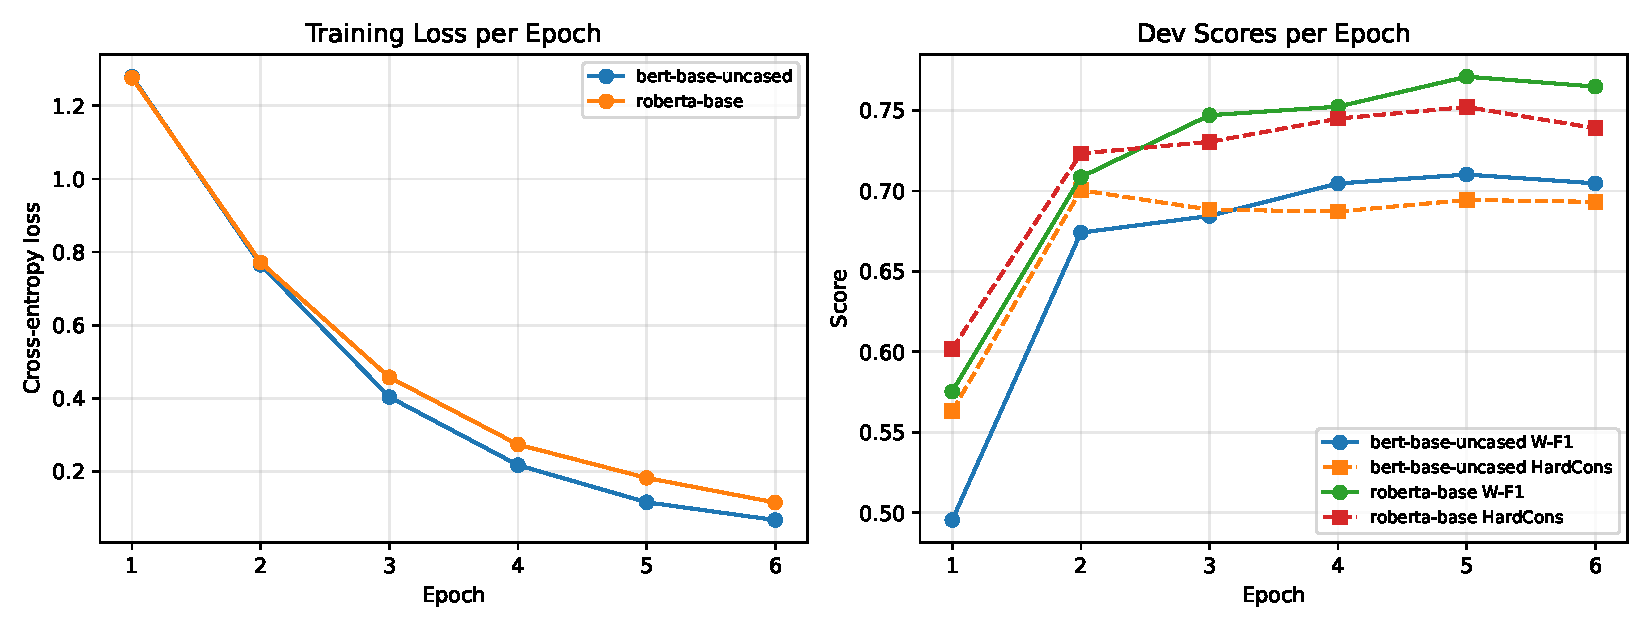
\includegraphics[width=\linewidth]{figures/training_curves.pdf}
\caption{Training loss (left) and development W-F1 and HardCons (right) per epoch, averaged over three seeds. Curves are diagnostic only and were not used for model selection.}
\label{fig:curves}
\end{figure}

\paragraph{Context.} On the public development-phase leaderboard of the task, the strongest Track~1 entries report W-F1 above 0.95 with SoftCons of 1.0, and the third entry reports 0.808 / 0.906 / 0.827. Our RoBERTa baseline (0.765 / 0.804 / 0.739) is below these but well above the fourth entry (0.510). This comparison is indicative only: development labels are public, so leaderboard systems may have been trained or tuned on them.

% =====================================================================
\section{Error Analysis}
\label{sec:errors}

We analyse seed~42 of each encoder and the strongest classical model.

\subsection{Confusion patterns}
Direction is largely handled by the encoders: both BERT and RoBERTa confuse \FWD{} with \BWD{} only twice in each direction, compared with 7 and 9 cases for the classical model. RoBERTa's errors concentrate at the boundary with \NEG{} (\cref{fig:confusion}): 20 \FWD{} and 20 \BWD{} rows are predicted as \NEG{}, 29 \EQ{} rows are predicted as \NEG{}, and 18 \NEG{} rows are predicted as \BWD.

\begin{figure}[t]
\centering
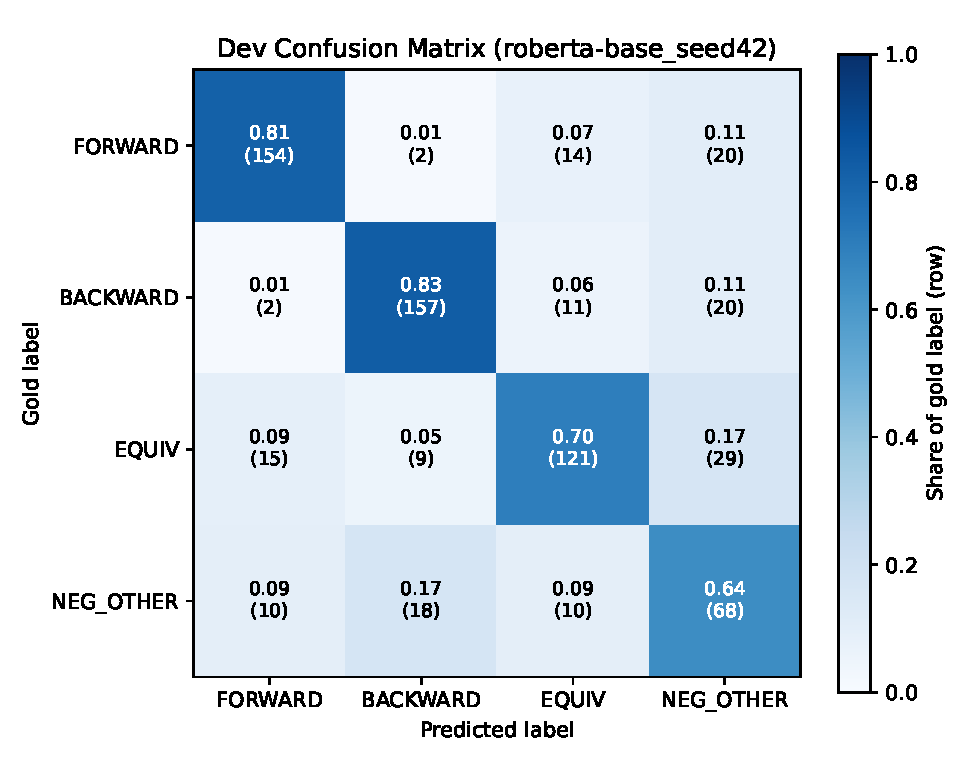
\includegraphics[width=0.55\linewidth]{figures/confusion_roberta.pdf}
\caption{Row-normalised development confusion matrix of RoBERTa-base (seed 42); counts in parentheses.}
\label{fig:confusion}
\end{figure}

\subsection{Pair-level outcomes}
\Cref{tab:pairs} classifies the 277 reversible pairs by the joint outcome of their two predictions.

\begin{table}[t]
\centering
\small
\begin{tabular}{lccc}
\toprule
Outcome & TF--IDF + feats & BERT & RoBERTa \\
\midrule
Both directions correct & 183 & 186 & \textbf{204} \\
Consistent but wrong & \textbf{54} & 28 & 16 \\
Direction-blind (same entailment label both ways) & 4 & 4 & 0 \\
\NEG{} predicted in one direction only & 35 & 47 & 42 \\
Other inconsistency & 1 & 12 & 15 \\
\bottomrule
\end{tabular}
\caption{Outcomes for the 277 reversible development pairs (seed 42 for the encoders).}
\label{tab:pairs}
\end{table}

The classical model owes much of its consistency to being consistently wrong (54 pairs), in line with the length-cue effect. The encoders produce far fewer such pairs; their main source of inconsistency is a \NEG{} prediction in only one orientation (42 pairs for RoBERTa), which automatically violates SoftCons and explains why their SoftCons is lower despite higher HardCons.

\subsection{Error categories}
We tag every misclassified row with a heuristic category (\cref{tab:errtypes}). For the classical model the largest category is confusion between \EQ{} and an entailment label (80 rows), followed by predictions that follow the length cue (68). For RoBERTa, length-cue errors fall to 38, a reduction of 44\%, and \EQ{}--entailment confusions to 34; the largest category becomes related pairs rejected as \NEG{} (69 rows).

\begin{table}[t]
\centering
\small
\begin{tabular}{lcc}
\toprule
Heuristic error category & TF--IDF + feats & RoBERTa \\
\midrule
Related pair rejected as \NEG & 56 & \textbf{69} \\
Followed length cue (longer side entails) & 68 & 38 \\
\EQ{} vs.\ entailment confusion & \textbf{80} & 34 \\
Contrastive/unrelated pair predicted as related & 43 & 19 \\
\bottomrule
\end{tabular}
\caption{Heuristic error categories (misclassified development rows).}
\label{tab:errtypes}
\end{table}

\subsection{Qualitative examples}
The \EQ{} pair ``a monochrome photograph'' / ``a black and white photo'' shows different behaviour across models. The length-only classifier predicts \EQ{} in both orientations, plausibly because the two phrases have the same number of characters (the signed character difference is zero). TF--IDF plus features predicts \BWD{} and \FWD{}, a consistent-but-wrong pair; BERT predicts \EQ{} in one direction and \NEG{} in the other; RoBERTa correctly predicts \EQ{} in both. The pair ``same-sex marriage'' / ``gay marriage'' (gold \EQ) is \FWD/\BWD{} for the length-only model, the best classical model and RoBERTa alike, and \FWD/\FWD{} for BERT.

Some RoBERTa errors involve distinguishing equivalence from one-way entailment. ``A black car'' $\rightarrow$ ``A black vehicle'' is labelled \FWD{} but predicted \EQ{}: the phrases are closely related, but a car is a vehicle whereas a vehicle need not be a car. Conversely, ``on green grass'' / ``on a lawn'' is labelled \EQ{} but predicted \FWD.

In the most frequent RoBERTa category, related pairs are rejected as \NEG{}, for example ``martial arts clubs'' / ``Martial Arts Schools'' and ``to pay off'' / ``of bribing'', both labelled \EQ{}. These near-paraphrases with different surface forms illustrate that the main remaining difficulty lies at the boundary between the reversible relations and \NEG.

Prepositional variation also remains challenging, echoing the findings of \citet{apaolaza2026assessing}. RoBERTa predicts \NEG{} for ``from Japan tunnel'' / ``in collapsed Japan tunnel'' (gold \BWD), and BERT predicts \BWD{} for ``out of the water'' / ``through the water'' (gold \NEG).

Finally, some disagreements expose the ambiguity of fine-grained labels. ``Australian senator'' / ``Australian lawmaker'' is labelled \NEG{}, although a \FWD{} reading is arguably defensible because a senator is a type of lawmaker. Cases like this limit what any single disagreement can tell us about a model.

\subsection{Segment information in BERT}
The preliminary BERT run without \texttt{token\_type\_ids} assigned the same entailment label to both orientations in 119 of the 190 \FWD/\BWD{} pairs, and its HardCons was 0.28. With segment IDs restored, the number of such direction-blind pairs falls to zero. Together with the revised training schedule, HardCons rose to $0.693\pm0.021$. The disappearance of direction-blind predictions is directly attributable to the segment information: BERT relies on segment embeddings to know which phrase comes first, whereas RoBERTa encodes order through separator tokens and positions only.

\subsection{Summary of failure modes}
The shallow models are consistent mostly because they follow a directional surface cue, and when the cue is misleading they are consistently wrong. The fine-tuned encoders have largely learned direction; they rarely mix up \FWD{} and \BWD{}. What they still get wrong is mainly the boundary with \NEG{}, and to a lesser extent equivalence versus one-way entailment and prepositional differences.

% =====================================================================
\section{Discussion}
\label{sec:discussion}

To answer the research question in one line: shallow cues get a model surprisingly far on consistency and not very far on correctness, while fine-tuned encoders reverse that balance. The result we found most telling is that the simplest informative model in the study, a classifier that only looks at phrase length, is also the most consistent one.

\paragraph{H1 (supported).} With four length features, LR achieves 0.464 W-F1 but 0.989 SoftCons, consistent with the EDA finding that about 77\% of \FWD{} rows place the longer phrase first. Signed length changes predictably under reversal, so the model produces compatible \FWD/\BWD{} pairs even when the relation is wrong, as for ``same-sex marriage'' / ``gay marriage''. The best classical model and RoBERTa make the same consistent-but-wrong prediction for this pair, and BERT predicts \FWD{} in both directions. Richer representations make this failure much rarer (54 consistent-but-wrong pairs for the classical model, 16 for RoBERTa), yet hard equivalence cases remain. On its own, a high SoftCons tells us very little about classification quality.

\paragraph{H2 (supported).} The best classical model reaches 0.620 W-F1 and 0.661 HardCons; RoBERTa reaches $0.765\pm0.002$ and $0.739\pm0.006$, and BERT $0.705\pm0.023$ and $0.693\pm0.021$. The largest gain is for \EQ{} (F1 0.515 $\rightarrow$ 0.725), consistent with the low lexical overlap of equivalent pairs: recognising a paraphrase takes lexical knowledge that surface matching lacks and pretraining provides.

\paragraph{H3 (supported).} \FWD/\BWD{} confusion becomes rare for the encoders (2 + 2 cases vs.\ 7 + 9 for the classical model). The dominant RoBERTa error is instead rejecting related pairs as \NEG{} (69 rows), and 42 reversible pairs receive \NEG{} in only one orientation.

\paragraph{Consistency versus correctness.} Across our models, SoftCons and correctness move in opposite directions. The length-only model has 0.989 SoftCons with 0.628 HardCons; RoBERTa has $0.804\pm0.011$ SoftCons with $0.739\pm0.006$ HardCons. The pair-level analysis explains why: the classical model produces 54 consistent-but-wrong pairs against 16 for RoBERTa, whereas RoBERTa's one-sided \NEG{} predictions lower its SoftCons. SoftCons alone would rank the length-only model first. HardCons ties coherence to correctness, and row-level F1 covers all four labels, including \NEG.

\paragraph{Limitations.}
(i) We evaluate on the development split rather than a blind test set; development labels are public, and seven development rows have exact text matches in training.
(ii) No hyperparameter search was performed. The encoder configuration was fixed after correcting the preliminary implementation issue, which limits tuning on the development set but means the models may not reach their best achievable performance.
(iii) MPS execution is not fully deterministic: repeated RoBERTa runs with the same seed and configuration differed by up to about 0.03 W-F1. We therefore report means over three seeds, although more seeds would give tighter estimates.
(iv) Error categories are assigned by heuristic rules and are neither manually verified nor mutually exclusive.
(v) A DeBERTa-v3 experiment was attempted but excluded because training produced NaN losses on the MPS backend.
(vi) Some fine-grained gold labels are arguable, which limits conclusions drawn from individual disagreements.

% =====================================================================
\section{Next Steps}
\label{sec:next}

\begin{enumerate}
  \item Predict both orientations of a pair jointly. Our classifiers label each row independently, and RoBERTa still produces 42 reversible pairs with \NEG{} in only one orientation. Scoring the two orientations together would let the model enforce, or at least encourage, \cref{eq:coherence}, and this source of inconsistency would disappear.
  \item Train with the reversal in mind. Feeding both orientations of a pair in the same batch, or adding a loss term that rewards $f(t_2,t_1)=\rev(f(t_1,t_2))$, may raise consistency without hurting accuracy. Reverse training \citep{golovneva2024reverse} is a natural place to start.
  \item Improve \NEG{}, which remains the weakest class (RoBERTa F1 0.565) and the largest error category. Class weighting is the simple option; modelling the original PhrasIS relations behind \NEG{} is the more interesting one.
  \item Run DeBERTa-v3, which should be evaluated in a CUDA environment where it trains stably, and submit the final systems to the blind test phase to see whether the development findings hold.
\end{enumerate}

\bibliographystyle{plainnat}
\bibliography{references}

\end{document}
